\section{Design of PCStream}
In this section, we describe in detail the proposed automatic stream management
technique, called \textit{PCStream}.  First, we explain a mechanism that
automatically obtains the program context (PC) value at runtime, and then
describe how multiple write streams with different PC values are combined and
delivered to an SSD. Finally, we introduce an additional technique that further
optimizes PCStream.

\subsection{Design overview}
Figure~\ref{fig:architecture} shows the overall architecture of PCStream.  When
the write system call handler is called from the user process, it passes the
user process information to the PC Extractor module.  Then the PC value is
extracted from the call stack of the writing process by the proposed method
which will be explained in the following subsection.  In order to analyze the
lifetime of PCs, we need to maintain the written time and the update/delete
time of the data for each PC.  The lifetime of data starts when they are
written for the first time, and ends when they are updated or deleted.  The
Lifetime Monitor module gets LBAs from the write handler to maintain the
written time or update time of the data written to the address.  When we get
TRIM command, the TRIM handler also passes the LBA on to the Lifetime Monitor
Module for keeping the delete time.  Together with the PC values and their
lifetimes, we can analyze the lifetime of the PCs of the system.  When the
number of PCs are greater than the number of streams, we cluster several PCs of
similar lifetime into a PC group to assign the same stream.  Finally, the
Stream Allocation module dynamically allocates PC group to the proper stream
according to the mapping policy.  The detailed mapping policy will be described
in Section 3.3.

\begin{figure}[t]
	\centering
	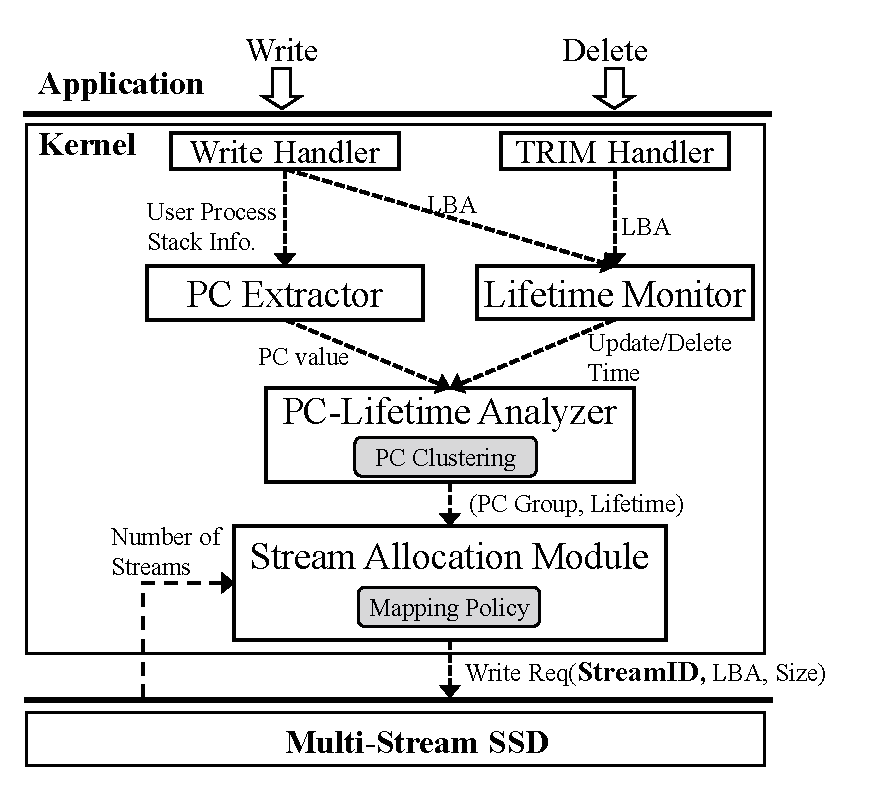
\includegraphics[width=0.8\linewidth]{figure/architecture2}
	\caption{An overall architecture of {\sf PCStream}}
	\label{fig:architecture}
	\vspace{-20pt}
\end{figure}

\subsection{Automatic PC Computation}
As mentioned earlier, we define the PC as the addition of instruction counter values along the 
execution path of the function call reaching the write. 
(In general, the function call process involves pushing the current instruction 
counter to the return address of the process stack.) 
Back tracing the stack and collect the return address can easily be done using the frame pointer register. 
However, when using the {\tt -fomit-frame-pointer} compile option of GCC, 
the general back tracing is impossible because frame pointer register is used for the general purpose~\cite{GCC}. 
Instead, we search from the top to bottom of the stack and regard the stack value 
belonging to the code area of the process as the return address. 

\begin{figure}[t]
	\centering
	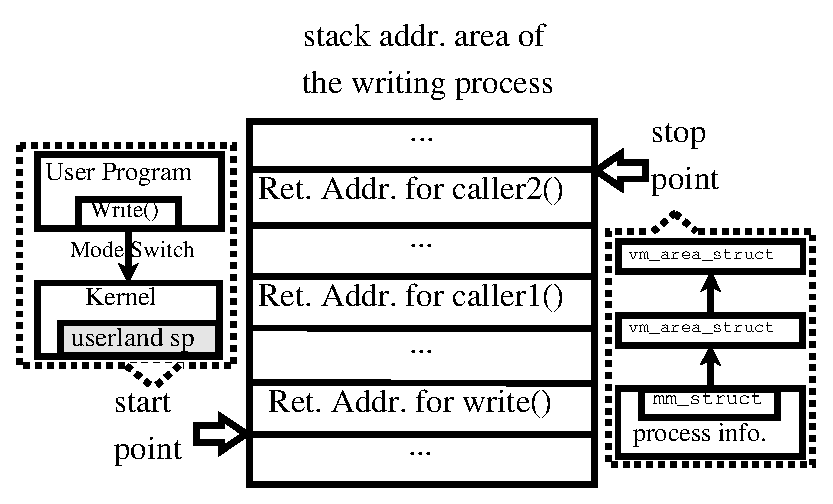
\includegraphics[width=1\linewidth]{figure/getpc}
	\vspace{-10pt}
	\caption{An automatic PC extraction method under compiler optimizations.}
	\label{fig:getpc}
	\vspace{-20pt}
\end{figure}

Figure~\ref{fig:getpc} shows the procedure. 
The start address of the user process stack search, depicted by (a) in Figure~\ref{fig:getpc},
is the stack pointer value of the user process 
which is maintained by the system call handler for returning from the kernel mode. 
The end address of the search, depicted by (b) in Figure~\ref{fig:getpc},
is the last address of the virtual memory management unit which
contains the user stack pointer value
from the process's virtual memory information. 
The scope of the code area of the process, depicted by (c) in Figure~\ref{fig:getpc},
is obtained from the virtual memory layout of the process information. 
In order to reduce the search time, we finish the searching 
when we find return addresses more than the threshold.
(Experimental results for various programs showed that different execution paths could be distinguished 
from each other only by a threshold value of 5 or less.)
The sum of all the address values found during the searching is used 
as the representative PC value of the context.
This process takes 300 to 400 nanoseconds on a 3.4 GHz CPU machine, 
so the time overhead is not huge.
Moreover, since we compute PC once per write system call,
the overhead can be distributed for long-length writes.

\subsection{Stream Allocation Policy}
In this paper, we focus on to show the feasibility of the PC-based approach, 
so we limits several factors of PCStream.
The number of application programs is limited to one, 
and we assume the SSD can support enough number of streams
to have 1:1 mapping policy for PCs and streams.
Since every PC is mapped to stream under the 1:1 mapping, 
we do not need to analyze the lifetime of PCs 
or dynamically allocate streams.
The implementation of those modules 
is left as a future work. 

For example, dynamic m:n mapping algorithm is
needed for responding to changes of
the application layer (increased number of PCs)
or the device layer (decreased number of streams).
For the PC clustering, we need to define the lifetime similarity of two PCs
and develop a clustering algorithm.
Also, we will develop the data structure
for the Lifetime Monitor to efficiently find a corresponding PC 
based on the discarded LBA because the deletion does not
make the write program context.

\subsection{Stream Refinement}
According to our observations, the lifetime of data is similar 
for contexts with simple operations such as log, as shown in section 2, 
but some contexts generate various lifetime data.
The compaction behavior of RocksDB belongs to a such context.
Compaction moves the flushed data to the different levels
of the LSM-tree~\cite{RocksDB}, 
so the data generated in one compaction context has 
different life characteristics depending on the target level.
Like RocksDB, LSM-tree-based DBs tend to have a longer 
data lifetime at lower levels~\cite{Level}.
Since the allocated capacity increases as the level goes down, 
the cycle of compaction, which deletes files, is long at low level.
In order to see the difference in the lifetime of each compaction target level,
we modified the RocksDB code to distinguish files according to the compaction level.
Figure~\ref{fig:compaction} shows the lifetime distribution of 
different compaction level data and compaction context data.

\begin{figure}[!t]
\centering
\hspace{1pt}
\subfloat[compaction:L2]{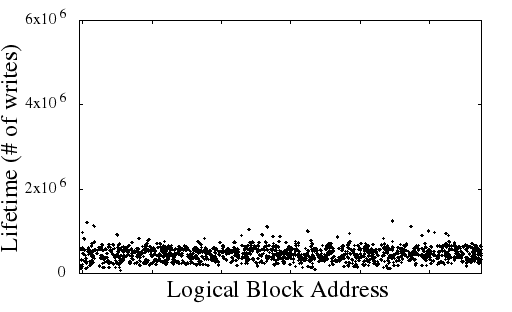
\includegraphics[width=0.23\textwidth]{figure/type_4b}}  % data from 4/03040047
\subfloat[compaction:L3]{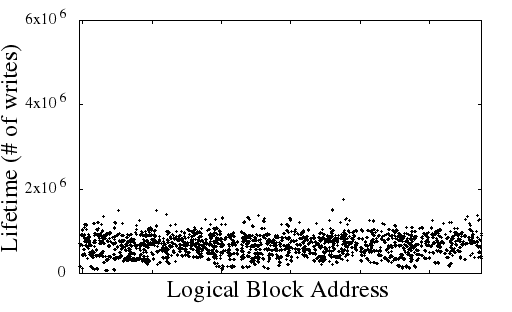
\includegraphics[width=0.23\textwidth]{figure/type_5b}}
\hfill
\vspace{-10pt}
\subfloat[compaction:L4] {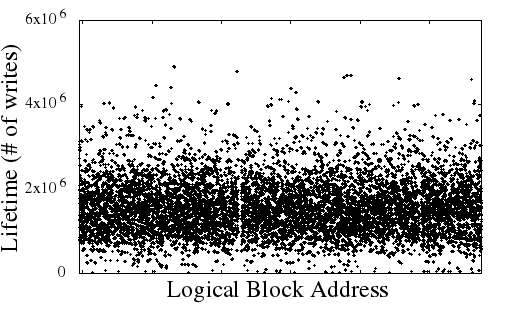
\includegraphics[width=0.23\textwidth]{figure/type_6b}}
\subfloat[PC ID: \#4]{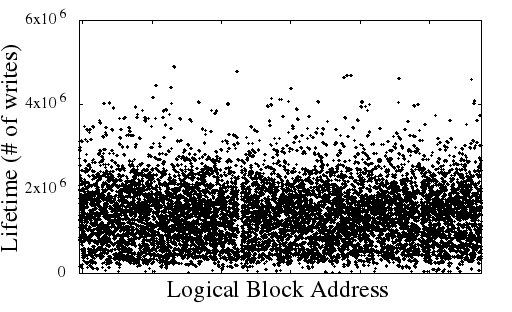
\includegraphics[width=0.23\textwidth]{figure/pc_3b}}
\vspace{-10pt}
\caption{The lifetime distribution of compaction context.} 
\label{fig:compaction}
\vspace{-25pt}
\end{figure}

Level 2 data in Figure~\ref{fig:compaction}(a) and 
level 3 data in Figure~\ref{fig:compaction}(b) seem to have 
a limited lifetime due to the frequent compaction.
On the other hand, because of the long compaction period 
due to the largest space of LSM-tree's lowest level, 
the lifetime is longer than other levels as shown in ~\ref{fig:compaction}(c).
Also, since the target file of the compaction is determined 
by the range of key values of the file~\cite{RocksDB}, 
the previously created file can be deleted 
by participating in the compaction. 
Therefore, the data stored at the lowest level has a very wide lifetime.
However, since all of these data are created in the same context, 
PC 4 can not distinguish any data of the compaction as shown in ~\ref{fig:compaction}(d).
In order to overcome the limitation of PC-based data classification,
we suggest a new optimization technique for multi-stream SSD 
rather than asking application to differentiate the compaction function according to its level.

Basically, the reason for distinguishing data of a similar lifetime is 
to match the timing of data invalidation. 
If long-lived data is gathered together excluding short-lived data, 
there would be no significant impact on WAF. 
So if we store the long-lived data separately even after 
the data is written to the wrong stream, 
we can greatly reduce the side effects of the limitation. 
Therefore, we consider a valid page copied during the GC 
as a misplaced long-lived data 
and allocate a separate substream to accommodate it. 
For example, if a PC with various lifetimes is assigned to stream A, 
we define stream A' as a substream of A and 
move the valid page of stream A to stream A' during GC. 
This prevents long lifetime data of stream A from being repeatedly copied 
by GC.



